\chapter{Análisis General}\label{ch:Análisis_General}

\section{Metodología}
Para la creación de este trabajo se opto por el modelo iterativo y creciente, dada la complejidad y amplitud del proyecto. Este enfoque permite abordar gradualmente la complejidad técnica, dividir el proyecto en etapas manejables y promover un enfoque centrado en el usuario, integrando retroalimentación continua para garantizar la satisfacción de los usuarios y optimizar la experiencia de aprendizaje. Además, facilita la adaptación a cambios y nuevos requisitos, asegurando una gestión eficaz del riesgo al identificar y mitigar problemas tempranamente, y enfatiza la validación y mejora continua del producto mediante pruebas y evaluaciones en cada iteración, asegurando la calidad y solidez del simulador final.

\begin{figure}[thbp]
    \centering
    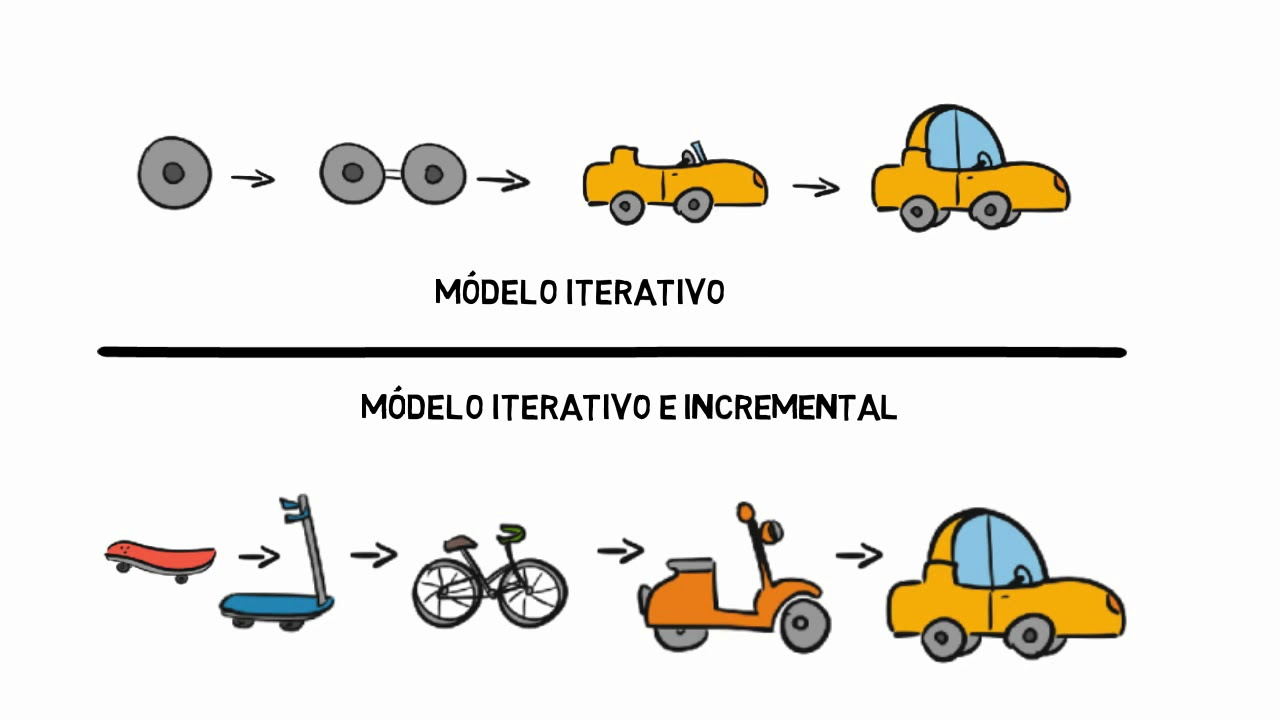
\includegraphics[width=0.7\textwidth, height = 6cm]{img/chapter03/iterativo incremental.jpg}
    \caption{Representación del modelo iterativo y modelo iterativo e incremental}
    \label{fig:iterativo_incremental}
\end{figure}

\textit{\textbf{Fase Preliminar:}} Diseño y Planificación (Iteración 0)
\begin{itemize}
    \item \textbf{Definición Detallada de Experimentos:} Elaboración de protocolos experimentales para los cuatro experimentos seleccionados (Reloj de Yodo, Sol de Fósforo, Síntesis de Cloruro de Amonio, Reacción Bromo-Aluminio), especificando reactivos, cantidades, procedimientos y resultados esperados.
    \item \textbf{Configuración del Entorno de Desarrollo:} Instalación y configuración de Unity (motor de videojuego), Blender (modelado 3D), Gimp (edición de imágenes) y entorno de programación C\#. Familiarización con las herramientas.
    \item \textbf{Definición del Alcance del Proyecto:} Establecimiento preciso de objetivos, funcionalidades, público objetivo, restricciones y plataforma de destino (Oculus Quest 2 y Meta Quest Pro).
    \item \textbf{Integración del SDK de Oculus:} Configuración del proyecto Unity para realidad virtual, integración del SDK de Oculus y pruebas de compatibilidad iniciales.
    \item \textbf{Implementación Básica del Seguimiento de Manos:} Habilitación y configuración inicial del sistema de seguimiento de manos en Unity, con pruebas preliminares de interacción
\end{itemize}

\textit{\textbf{Iteración 1:}} Base del Simulador y Tabla Periódica Interactiva
\begin{itemize}
    \item\textbf{Desarrollo del Entorno Virtual:} Creación del escenario del laboratorio y configuración de iluminación y ambiente.
    \item\textbf{Tabla Periódica Interactiva:} Diseño e implementación de una interfaz de tabla periódica funcional, con selección de elementos, visualización de información básica (nombre, símbolo, número atómico, masa atómica) y modelos 3D interactivos de isótopos.
    \item\textbf{Modelado 3D de Isótopos:} Diseño y creación de modelos 3D de los isótopos principales de cada elemento.
    \item\textbf{Integración de Modelos 3D:} Importación y configuración de los modelos 3D en Unity, estableciendo la conexión con la tabla periódica interactiva.
    \item\textbf{Modelado de Materiales y Herramientas:} Diseño y modelado 3D de materiales y herramientas de laboratorio (matraces, tubos de ensayo, mecheros, etc.) con funcionalidad básica de manipulación.
\end{itemize}

\textit{\textbf{Iteración 2:}} Tutorial Interactivo
\begin{itemize}
    \item \textbf{Diseño del Tutorial:} Elaboración de un guion detallado con objetivos de aprendizaje, pasos secuenciales e interacciones del usuario. Diseño de elementos visuales (flechas, indicaciones, animaciones) para guiar al usuario.
    \item \textbf{Implementación del Tutorial:} Programación de la lógica del tutorial en Unity, incluyendo instrucciones de voz (grabadas) y manejo de interacciones con objetos virtuales.
    \item \textbf{Pruebas y Ajustes:} Evaluación del tutorial con usuarios, realizando ajustes en base a la retroalimentación recibida para garantizar claridad, eficacia y usabilidad.
\end{itemize}
\newpage
\textit{\textbf{Iteraciones 3-6:}} Desarrollo de Experimentos
Para cada uno de los cuatro experimentos (De Básico a Ácido, La lampara de magnesio, Nieve Química, La Bruja de Bromo), se seguirá el siguiente proceso iterativo:
\begin{itemize}
    \item \textbf{Modelado 3D:} Creación de modelos detallados de reactivos y productos específicos del experimento.
    \item \textbf{Animaciones:} Desarrollo de animaciones realistas para representar las reacciones químicas y los cambios físicos observados.
    \item \textbf{Lógica del Experimento:} Implementación de la secuencia de pasos guiados, simulación de reacciones químicas (incluyendo cálculos de concentraciones, tiempos de reacción y cambios de color), evaluación formativa del desempeño del usuario y retroalimentación detallada.
    \item \textbf{Pruebas:} Pruebas del experimento para asegurar la precisión científica, la funcionalidad y la usabilidad.
\end{itemize}

\begin{figure}[thbp]
    \centering
    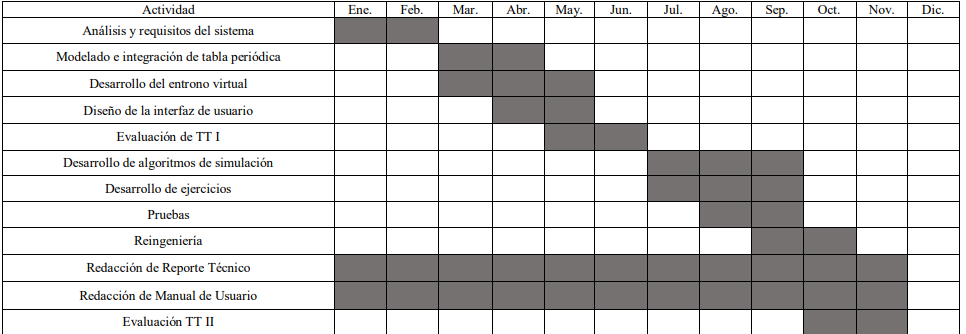
\includegraphics[width=0.8\textwidth, height = 7.5cm]{img/chapter03/Cronograma.png}
    \caption{Cronograma de Actividades}
    \label{fig:Cronograma}
\end{figure}

\section{Análisis de Requerimientos}
\subsection{Requerimientos Funcionales}
\begin{enumerate}[RF1.]
    \item \textit{Menú Principal: }El sistema presentará un menú principal intuitivo y organizado al inicio de la ejecución. Este menú proporcionará acceso a las funcionalidades del sistema, incluyendo un tutorial, selección de experimentos.
    \item \textit{Selección de Elementos}
    \begin{enumerate}[{RF2.}1.]
        \item \textit{Tabla Periódica Interactiva: }El sistema incorporará una tabla periódica interactiva que permita al usuario visualizar todos los elementos químicos de forma organizada.
        \item \textit{Selección Visual de Elementos: }El usuario podrá seleccionar elementos directamente desde la tabla periódica interactiva con un toque. 
        \item \textit{Visualización de Información Detallada: }Al seleccionar un elemento, se mostrará una ventana emergente con información detallada sobre el mismo, incluyendo su modelo atómico en 3D, descripción química y propiedades físicas y químicas. 
    \end{enumerate}
    \item \textit{Experimentación Virtual}
    \begin{enumerate}[{RF3.}1.]
        \item \textit{Instrucciones Paso a Paso:} El sistema guiará al usuario a través de cada experimento mediante instrucciones claras y concisas que detallen la cantidad de reactivos a utilizar y el procedimiento a seguir.
        \item \textit{Simulación de Reacciones: }El sistema simulará la reacción química entre los elementos seleccionados, siguiendo principios químicos establecidos.
        \item \textit{Observación de Efectos:} El usuario podrá observar los efectos de la reacción química en el entorno virtual, como la formación de nuevos compuestos, la liberación de gases o cambios de color.
    \end{enumerate}
\end{enumerate}
\subsection{Requerimentos No Funcionales}
\begin{enumerate}[RNF1.]
    \item \textit{Rendimiento}
    \begin{enumerate}[{RNF1.}1.]
        \item \textit{Fluidez Gráfica: }El sistema debe exhibir una tasa de cuadros por segundo (FPS) constante y superior a 60 FPS, para garantizar una experiencia de usuario inmersiva y sin interrupciones.
        \item \textit{Tiempo de Respuesta: }El sistema debe presentar un tiempo de respuesta mínimo a las acciones del usuario, minimizando los retrasos y garantizando una interacción dinámica y receptiva.
    \end{enumerate}
    \item \textit{Usabilidad}
    \begin{enumerate}[{RNF2.}1.]
        \item \textit{Interfaz Intuitiva: }La interfaz de usuario debe seguir principios de diseño intuitivos y accesibles, utilizando elementos visuales claros, jerarquías de información bien definidas y una navegación sencilla. 
        \item \textit{Navegación Sencilla: }La interfaz de usuario debe seguir principios de diseño intuitivos y accesibles, utilizando elementos visuales claros, jerarquías de información bien definidas y una navegación sencilla. 
        \item \textit{Retroalimentación Clara: }El sistema debe proporcionar retroalimentación clara y concisa al usuario sobre sus acciones e interacciones dentro del entorno virtual. 
    \end{enumerate}
\end{enumerate}
\newpage
\subsection{Reglas de Negocio}
El prototipo de simulador de laboratorio de química inorgánica en realidad virtual se regirá por las siguientes reglas de negocio: 

\begin{enumerate}[{RN-}01. ]
    \item \textit{\textbf{Selección de Elementos: }}
    \begin{itemize}
        \item Un elemento químico se considera seleccionado cuando el usuario toca su ficha en la tabla periódica con su dedo índice. 
        \item Solo se puede seleccionar un elemento a la vez. Si se selecciona un elemento que ya existe en la escena, este se destruye y se crea uno nuevo en la zona designada. 
        \item La GUI se actualizará con la información del elemento seleccionado. 
    \end{itemize}

    \item \textit{\textbf{Creación de Compuestos: }}
    \begin{itemize}
        \item Para crear un compuesto, el usuario debe llevar los elementos necesarios a la zona de creación. 
        \item El sistema verificará si cada elemento es correcto para el compuesto en dos ocasiones: al seleccionarlo y al entrar en la zona de creación. 
        \item Si un elemento es incorrecto, el sistema notificará al usuario mediante un mensaje de voz y texto, y le indicará que lo lleve a la zona de desecho. 
        \item El compuesto se formará solo cuando todos los elementos necesarios estén presentes en la zona de creación. 
        \item Una vez creado el compuesto, se mostrará su modelo 3D en el área de experimentación y se actualizará la GUI correspondiente. 
    \end{itemize}

    \item \textit{\textbf{Interacción con Objetos: }}
    \begin{itemize}
        \item El usuario puede agarrar, mover y soltar compuestos, instrumental y elementos utilizando el seguimiento de manos (hand tracking). 
        \item La interacción con objetos estará limitada a las acciones permitidas en cada etapa del experimento. 
    \end{itemize}

    \item \textit{\textbf{Simulación de Reacciones: }}
    \begin{itemize}
        \item La simulación de reacciones químicas presentará efectos visuales básicos, como cambios de color y liberación de gases, priorizando la comprensión de los conceptos fundamentales sobre el realismo detallado.
    \end{itemize}
    
    \item \textit{\textbf{Etapas del Experimento: }}
    \begin{itemize}
        \item Cada experimento se dividirá en cinco etapas: presentación, balanceo de ecuación, selección de elementos y creación de compuestos, desarrollo y simulación, y explicación de resultados y conclusiones. 
        \item El usuario avanzará a la siguiente etapa solo después de completar exitosamente la etapa anterior. 
        \item En la etapa de desarrollo y simulación, el usuario seguirá instrucciones paso a paso y realizará las acciones necesarias para completar el experimento. 
    \end{itemize}
    \newpage
    \item \textit{\textbf{Retroalimentación al Usuario: }}
    \begin{itemize}
        \item El sistema proporcionará retroalimentación visual y auditiva al usuario en cada etapa del experimento. 
        \item En caso de errores, se mostrarán mensajes claros y concisos en la GUI indicando el problema y cómo solucionarlo. 
    \end{itemize}
    
    \item \textit{\textbf{Navegación:}}  
    \begin{itemize}
        \item Al finalizar un experimento, el usuario será redirigido automáticamente al escenario de bienvenida. 
        \item Desde el escenario de bienvenida, el usuario podrá seleccionar otro experimento o repetir el tutorial.
    \end{itemize}

    \item \textit{\textbf{Eliminación de Elementos: }}
    \begin{itemize}
        \item Los elementos químicos y compuestos pueden ser eliminados del área de trabajo arrastrándolos a la zona de desecho. 
        \item El sistema verificará si el elemento o compuesto puede ser desechado en ese momento del experimento. 
    \end{itemize}

    \item \textit{\textbf{Balanceo de Ecuaciones:}} 
    \begin{itemize}
        \item En la etapa de balanceo de ecuaciones, el usuario deberá ajustar los coeficientes estequiométricos de la reacción química para cumplir con la ley de conservación de la masa.   
        \item El sistema verificará si la ecuación está correctamente balanceada antes de permitir al usuario avanzar a la siguiente etapa. 
    \end{itemize}
    \item \textit{\textbf{Tutorial Interactivo: }}
    \begin{itemize}
        \item El tutorial guiará al usuario a través de las funciones básicas del simulador, incluyendo la selección de elementos, la creación de compuestos y la interacción con el instrumental. 
        \item El tutorial será opcional y podrá ser repetido en cualquier momento desde el menú principal. 
    \end{itemize}
\end{enumerate}

\subsection{¿Como debe venderse?}
Como una herramienta educativa y de entretenimiento inmersiva que permite a los usuarios explorar y experimentar con la química inorgánica de manera segura y divertida. El simulador ofrece una experiencia interactiva y visualmente atractiva, que permite a los usuarios manipular elementos químicos, realizar experimentos guiados y observar reacciones en tiempo real en un entorno de laboratorio virtual. 

Se puede distribuir de dos formas: 
\begin{itemize}
    \item\textit{\textbf{Versión demo gratuita:}} permitiendo a los usuarios potenciales experimentar con una selección limitada de experimentos y familiarizarse con la interfaz y el funcionamiento del simulador. 
    \item\textit{\textbf{Licencia completa:}} proporcionando acceso completo a todas las funcionalidades y experimentos disponibles en el simulador. 
\end{itemize}

El público objetivo del simulador incluye: 
\begin{itemize}
    \item Estudiantes de secundaria y nivel medio superior que cursan química. 
    \item Profesores de química que buscan herramientas innovadoras para sus clases. 
    \item Aficionados a la ciencia y entusiastas de la realidad virtual. 
    \item Museos y centros de ciencia que buscan ofrecer experiencias educativas interactivas. virtual.
\end{itemize}
\subsection{Limitaciones del Sistema}
El prototipo de simulador de laboratorio de química inorgánica en realidad virtual presentará las siguientes limitaciones inherentes a su diseño y alcance: 

\begin{itemize}
    \item \textbf{Ámbito Exclusivo en Química Inorgánica:} El simulador se circunscribe a la simulación de experimentos dentro del dominio de la química inorgánica, excluyendo otras ramas de la química, como la orgánica, la bioquímica o la fisicoquímica. 
    \item \textbf{Experimentación Guiada y Estructurada:} La experiencia del usuario se centra en experimentos predefinidos y guiados, priorizando la facilidad de uso y la comprensión de los conceptos fundamentales de la química inorgánica. No se contempla la posibilidad de realizar experimentos libres o personalizados en esta versión.

    \item \textbf{Limitaciones en el Realismo:} Aunque se busca la mayor fidelidad posible a la realidad, es importante destacar que el simulador ofrece una representación virtual de los fenómenos químicos. Algunas reacciones o propiedades químicas podrían ser simplificadas o idealizadas para facilitar la comprensión y el uso educativo, sin comprometer la validez de los conceptos aprendidos.
    \item \textbf{Plataformas Compatibles:} El simulador será compatible exclusivamente con los dispositivos de realidad virtual Oculus Meta Quest 2 y Oculus Meta Quest Pro. 
\end{itemize}
\newpage
\section{Tecnologías de Desarrollo}
\subsection{Modelado 3D y Animación}
\subsubsection{Blender}\\

Blender 3D es un software multiplataforma y gratuito especializado en el modelado, iluminación, renderizado, animación y creación de modelos 3D. También incluye composición digital utilizando nodos, edición de video, escultura y pintura digital.

El objetivo principal de Blender es generar imágenes 2D a partir de escenas 3D, utilizando diversos motores gráficos, tanto de pre-renderizado como de tiempo real, que vienen integrados por defecto. El programa ofrece una variedad de figuras geométricas primitivas, como curvas, mallas poligonales, vacíos y metaballs, además de una amplia gama de herramientas para modelado, renderizado, rigging, edición de video, audio, composición y animación.

Blender también incluye herramientas de animación avanzadas como cinemática inversa, deformaciones con armaduras o cuadrículas, vértices de carga y partículas estáticas. Además, proporciona características interactivas para el desarrollo de juegos, incluyendo detección de colisiones, simulaciones dinámicas, aplicación de físicas y lógica.

La interfaz gráfica OpenGL de Blender es uniforme y personalizable en las principales plataformas, y permite el uso de scripts en Python para automatizar y controlar varias tareas. Admite formatos gráficos como TGA, JPG, Iris, SGI y TIFF, e incluye simulaciones dinámicas para cuerpos blandos, partículas y fluidos. También cuenta con un sistema de partículas estáticas para simular cabello y pelaje, con opciones avanzadas de shaders para texturas realistas.

Desde su creación en 2001, Blender ha sido reconocido por su constante desarrollo y mejoras, proporcionando a los usuarios una experiencia única y en evolución.\\

\begin{figure}[thbp]
    \centering
    \includegraphics[width=0.5\textwidth, height = 5cm]{img/chapter03/Modelo_Atómico.png}
    \caption{Modelo de un átomo en Blender}
    \label{fig:atomo}
\end{figure}

\subsubsection{Gimp}
Este software de manipulación de imágenes ha experimentado una notable evolución a lo largo del tiempo. Utiliza GTK como biblioteca de controles gráficos.

Permite trabajar con imágenes en capas, lo que facilita la modificación independiente de cada objeto en la imagen. Las capas pueden organizarse en una pila, subiendo o bajando de nivel para facilitar la edición. Cada capa tiene su propia visibilidad y nivel de transparencia, y hay numerosas formas de combinar las relaciones entre ellas.

Además, es posible producir imágenes de manera completamente automatizada y no interactiva, así como realizar un procesamiento por lotes que cambia colores o convierte series de imágenes. Para tareas automatizadas más simples, se recomienda utilizar un paquete como ImageMagick.

\textit{\textbf{Imágenes}}\\
Una imagen en GIMP puede ser más compleja de lo que parece. No es solo un dibujo en un lienzo, sino una pila de capas, una máscara de selección, un conjunto de canales y rutas.

Cuenta con un sistema de gestión de memoria avanzado basado en bloques de píxeles, lo que permite manejar imágenes muy grandes sin dificultad.

\textit{\textbf{Capas}}\\
Una imagen con capas es similar a un fajo de papeles transparentes apilados. Se puede dibujar en cada papel y ver el contenido de otras hojas a través de las áreas transparentes. También es posible mover una hoja en relación con las demás.

Una imagen en GIMP puede contener muchas capas, incluso docenas. Las capas no tienen que ser opacas ni cubrir toda la extensión de la imagen, por lo que se puede ver más que la capa superior, observando elementos de otras capas.

\textit{\textbf{Canales}}\\
Los canales son útiles cuando se trabaja en una imagen que necesita ajustes en un color específico. Ver los canales como máscaras permite restringir la salida del color que el canal representa. Usando filtros en la información del canal, se pueden crear muchos efectos variados y sutiles sobre una imagen. Con estos canales, es posible crear otros canales, conocidos como máscaras de canal.
\subsection{Motor de Videojuegos}
\subsubsection{Unity}
Unity es una plataforma líder en el desarrollo de juegos, compatible con múltiples plataformas, ampliamente utilizada para crear experiencias interactivas tanto en 3D como en 2D. Su ecosistema completo, que incluye un amplio conjunto de herramientas y una comunidad activa, facilita la creación de simulaciones de realidad virtual realistas, la interacción natural con elementos virtuales y el desarrollo de interfaces de usuario intuitivas.

El entorno integrado de Unity está compuesto por diversas partes y componentes que permiten el desarrollo de simuladores. Está desarrollado en C\#, un lenguaje de programación multiparadigma que, al ser de acceso libre, fomenta la creación de contenido por parte de la comunidad y la creación de sus propias librerías.

C\# es la tercera versión de C y una mejora respecto a C++, lo que simplifica la exportación y comunicación con programas escritos en estos lenguajes sin necesidad de una interfaz compleja.

\subsubsection{C\#}
C\# es un lenguaje de programación que se centra en componentes, está orientado a objetos y garantiza la seguridad de tipos. Esto permite a los desarrolladores crear una variedad de aplicaciones seguras y robustas que se ejecutan en el entorno .NET. Es especialmente adecuado para la creación y utilización de componentes de software, y ofrece características que respaldan nuevas cargas de trabajo y prácticas de diseño de software en evolución. En esencia, C\#  es un lenguaje orientado a objetos.

\subsubsection{GameObject}
Los GameObject son elementos esenciales en Unity, ya que pueden representar diversos elementos como avatares, objetos o el escenario mismo. Por sí solos, estos elementos no realizan ninguna función, pero actúan como contenedores para sus Componentes.

\begin{figure}[thbp]
    \centering
    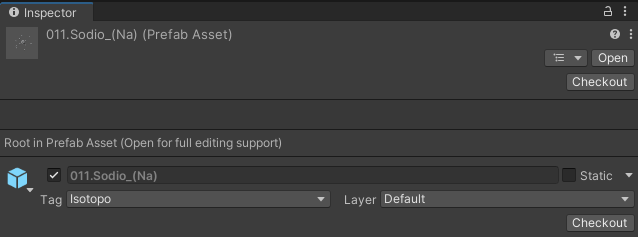
\includegraphics[width=0.7\textwidth, height = 4cm]{img/chapter03/Game_Object.png}
    \caption{Game Object en Unity}
    \label{fig:game_object}
\end{figure}

\subsubsection{Componentes}
Los componentes son los que definen el comportamiento de cada GameObject en el juego. No existe un límite establecido en cuanto a la cantidad de componentes que puede tener un objeto.

\begin{figure}[thbp]
    \centering
    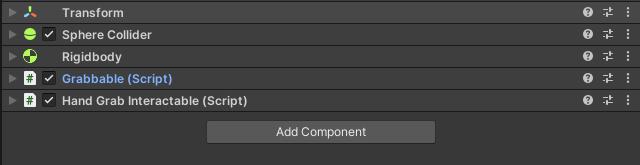
\includegraphics[width=0.7\textwidth, height = 4cm]{img/chapter03/Components.png}
    \caption{Componentes de un Elemento en Unity}
    \label{fig:components}
\end{figure}

\subsubsection{Script}
El Script es un componente diseñado por el usuario para realizar una acción específica en el juego. Consiste en una secuencia de líneas de comandos escritas principalmente en C\# o en UnityScript. Sin embargo, otros lenguajes .NET pueden ser utilizados con Unity si son compilados en un DLL compatible.

Los Scripts permiten activar eventos en su juego, modificar propiedades del Componente en tiempo real y responder al input del usuario de la manera que desee. Puede crear un nuevo script desde el menú ``Create'' en la parte superior izquierda del panel del Proyecto, o seleccionando ""Assets \verb|>| Create \verb|>| C\# Script"" desde el menú principal.

Cuando se adjunta un componente script a un GameObject, se crea una nueva instancia del objeto definido por el plano. Es importante tener en cuenta que un script solo define un plano para un componente; su código no se activará hasta que una instancia del script sea adjuntada al GameObject.

\subsubsection{ScriptableObject}
ScriptableObject es una clase en Unity que permite almacenar grandes cantidades de datos compartidos independientes de las instancias de script. A diferencia de SerializableObject, esta clase está diseñada específicamente para este propósito y no debe confundirse con ella.

Cuando se utiliza ScriptableObject, los datos se almacenan por referencia en lugar de por valor, lo que significa que las instancias de ScriptableObject mantienen los datos y las instancias de script solo contienen referencias a estos datos. Esto ayuda a reducir el uso de memoria al evitar la duplicación de valores.

Un caso de uso común para ScriptableObject es definir conjuntos de datos conectables, como en el caso de una tienda NPC en un juego RPG, donde cada zona puede ofrecer diferentes tipos de ítems para la venta. Los objetos de ScriptableObject personalizados pueden definir estos conjuntos de datos, lo que permite una fácil configuración y personalización del juego.
\begin{figure}[thbp]
    \centering
    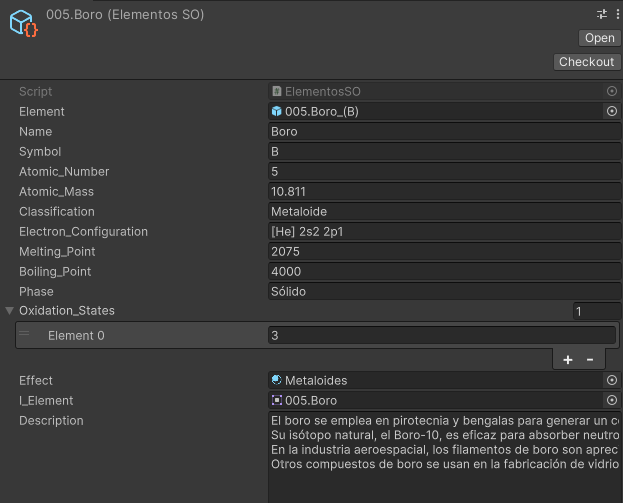
\includegraphics[width=0.6\textwidth, height = 7cm]{img/chapter03/ScriptableObject.png}
    \caption{ScriptableObject de un Elemento en Unity}
    \label{fig:components}
\end{figure}
\newpage
\subsection{Integración de Oculus Meta Quest 2 y Oculus Meta Quest Pro}
Meta Quest 2 y Meta Quest Pro son dispositivos de realidad virtual (VR) desarrollados por Meta Platforms (anteriormente Facebook), cada uno diseñado para satisfacer necesidades y expectativas específicas de los usuarios.

\textit{Meta Quest 2:} Lanzado en 2020, este dispositivo autónomo ofrece una experiencia de VR inmersiva sin necesidad de una PC externa, proporcionando un rendimiento fluido en la mayoría de aplicaciones y juegos disponibles en su plataforma, brindando una experiencia visual de alta calidad.

\begin{figure}[thbp]
    \centering
    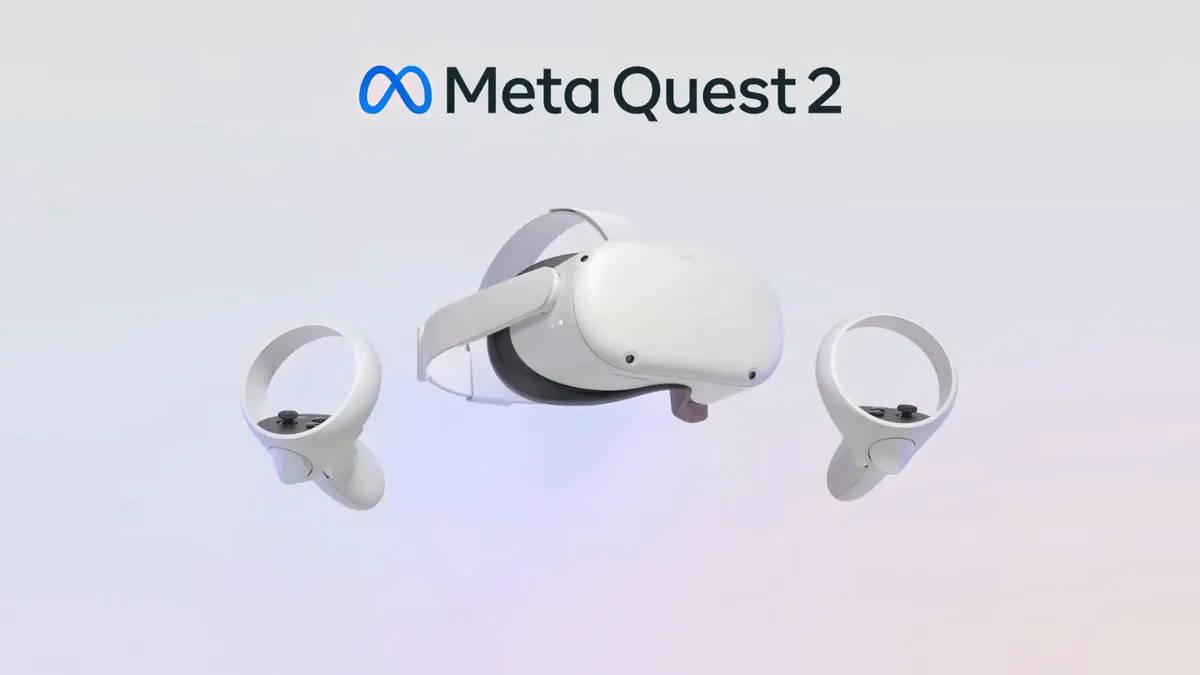
\includegraphics[width=0.5\textwidth, height = 4cm]{img/chapter03/Meta_Quest_2.png}
    \caption{Oculus Meta Quest 2}
    \label{fig:Oculus_Meta_Quest_2}
\end{figure}

\textit{Meta Quest Pro:} Lanzado en 2022, este dispositivo de gama alta está orientado a profesionales y entusiastas de la VR, ofrece un rendimiento superior y capacidades avanzadas. Además, incorpora seguimiento ocular y facial, así como cámaras de alta resolución, que permiten una interacción más natural y expresiva en entornos virtuales, y habilitan funciones de realidad mixta.

\begin{figure}[thbp]
    \centering
    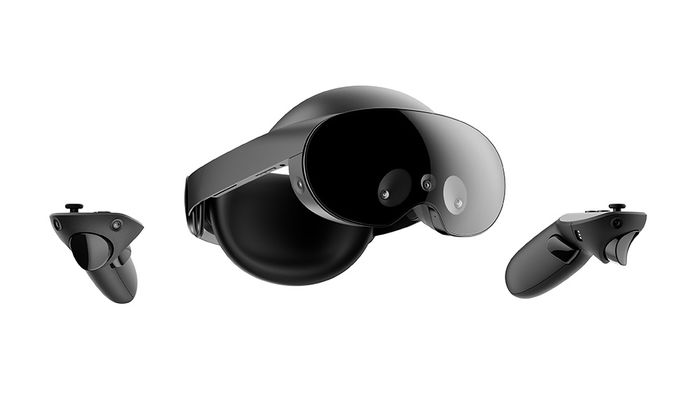
\includegraphics[width=0.5\textwidth, height = 4cm]{img/chapter03/Meta_Quest_Pro.png}
    \caption{Oculus Meta Quest Pro}
    \label{fig:Oculus_Meta_Quest_Pro}
\end{figure}

\textit{SDK de Oculus}

El SDK de Oculus proporciona las herramientas y bibliotecas necesarias para integrar el simulador con las gafas VR Oculus Meta Quest 2 y Oculus Meta Quest Pro de manera nativa. Permite el seguimiento preciso de la cabeza y el movimiento de las manos, la representación 3D estereoscópica de alta calidad y la interacción natural con elementos virtuales, creando una experiencia de realidad virtual inmersiva y atractiva.

\begin{longtable}{|>{\centering\arraybackslash}m{.2\textwidth}|>{\centering\arraybackslash}m{.4\textwidth}|>{\centering\arraybackslash}m{.4\textwidth}|}
    \hline
    \rowcolor{blue_escom}
    Característica & Meta Quest 2 & Meta Quest Pro  \\
    \hline
    \endfirsthead

    \hline
    \rowcolor{blue_escom}
    Característica & Meta Quest 2 & Meta Quest Pro  \\
    \hline
    \endhead

    \multicolumn{3}{r}{\textit{Continúa en la siguiente página}} \\
    \endfoot

    \endlastfoot

    \cellcolor{column_color}Resolución por Ojo & 1832x1920 pixeles & 1800x1920 pixeles \\
    \hline
    \cellcolor{column_color}Frecuencia de Actualizaión & 72-90 Hz & 72-90 Hz \\
    \hline
    \cellcolor{column_color}Procesador & Qualcomm Snapdragon XR2 & Qualcomm Snapdragon XR2+ \\
    \hline
    \cellcolor{column_color}RAM & 6 GB & 12 GB \\
    \hline
    \cellcolor{column_color}Almacenamiento & 128 GB / 256 GB & 256 GB \\
    \hline
    \cellcolor{column_color}Seguimiento Ocular y Facial & ✗ & ✓ \\
    \hline
    \cellcolor{column_color}Cámaras & 4 & 10 \\
    \hline
    \cellcolor{column_color}Realidad Mixta & ✗ & ✓ \\
    \hline
    \cellcolor{column_color}Duración de la batería & 2-3 horas & 2-3 horas \\
    \hline
    \cellcolor{column_color}Precio aproximado & \$299 USD (128 GB) / \$399 USD (256 GB) & \$999 USD \\
    \hline

  \caption{Comparación de especificaciones entre Oculus Meta Quest 2 y Oculus Meta Quest Pro}
  \label{tab:Quest_2_vs_Quest_Pro}
\end{longtable}
\newpage
\subsection{Handtracking}
El seguimiento de manos (hand tracking) es una tecnología que permite la detección y seguimiento en tiempo real de los movimientos de las manos del usuario a través de dispositivos equipados con cámaras, como las gafas de realidad virtual Meta Quest. Esta tecnología se basa en el análisis de imágenes capturadas por las cámaras, identificando puntos clave en las manos y rastreando su movimiento a medida que el usuario las desplaza.
El seguimiento de manos ofrece una modalidad de interacción más natural e intuitiva con dispositivos y entornos virtuales, eliminando la necesidad de controladores físicos.

\textbf{En Realidad virtual (VR) y realidad mixta:} Permite una interacción más inmersiva y realista con entornos virtuales, mejorando la experiencia del usuario en juegos, simulaciones y aplicaciones de entrenamiento.\\
\begin{figure}[thbp]
    \centering
    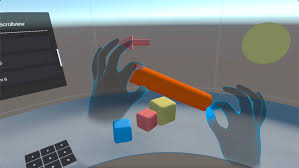
\includegraphics[width=0.5\textwidth, height = 4cm]{img/chapter03/hand_tracking.jpeg}
    \caption{Ejemplo de Handtracking}
    \label{fig:Handtracking}
\end{figure}
\section{Análisis Económico}
\subsection{Análisis por Puntos de Función}
Métrica de punto de función La métrica de punto de función (PF) puede usarse de manera efectiva como medio para medir la funcionalidad que entra a un sistema. 

Para obtener el PF vamos a considerar los valores de dominio de información que se definen de la siguiente forma:  

\textit{\textbf{Número de entradas externas (EE): 5}}
\begin{itemize}
    \item Elegir experimento/tutorial (Simple)
    \item Seleccionar elemento (Simple)
    \item Eliminar elemento (Simple) 
    \item Crear compuesto (Simple) 
    \item Interactuar con instrumental (Simple)
\end{itemize}
\textit{\textbf{Número de salidas externas (SE): 3  }}
\begin{itemize}
    \item Visualización del experimento (Complejo)
    \item Resultados del experimento (Complejo)
    \item Visualización del Entorno de Laboratorio (Promedio)
    \item Visualización de Elementos y Compuestos (Promedio)
    \item Indicaciones visuales y auditivas (Promedio) 
\end{itemize}
\textit{\textbf{Número de consultas externas (CE): 0  }}

\textit{\textbf{Número de archivos lógicos internos (ALI): 3  }}
\begin{itemize}
    \item Datos de experimentos (Promedio)
    \item Datos de elementos (Promedio)
    \item Datos de compuestos (Promedio)
\end{itemize}
\textit{\textbf{Número de archivos de interfaz externos (AIE): 0  }}

\begin{table}[H]
  \centering
  \begin{tabular}{|>{\centering\arraybackslash}m{.2\textwidth}|>{\centering\arraybackslash}m{.13\textwidth}>
  {\centering\arraybackslash}m{.015\textwidth}>{\centering\arraybackslash}m{.095\textwidth}>{\centering\arraybackslash}m{.095\textwidth}>{\centering\arraybackslash}m{.095\textwidth}>{\centering\arraybackslash}m{.015\textwidth}>{\centering\arraybackslash}m{.07\textwidth}|}
    \hline
    \rowcolor{blue_escom}
     &\multicolumn{7}{c|}{\parbox[0.53\textwidth]{0.515\textwidth}{\centering\textbf{Factor Ponderado}}}\\
    \cline{2-8} 
    
    \multirow{-2}{.2\textwidth}{\cellcolor{blue_escom} \centering \textbf{Valor de dominio de información}} & Conteo & & Simple & Promedio & Complejo & & Total\\ 
    \hline
    \cellcolor{column_color}Entradas Externas (EE) & 5 Simples & * & 3 & 4 & 6 & = & 15 \\
    \hline
    \cellcolor{column_color}Salidas Externas (SE) & 2 Complejos, 3 Promedio & * & 4 & 5 & 7 & = & 29 \\
    \hline
    \cellcolor{column_color}Consultas Externas (CE) & 0 & * & 3 & 4 & 6 & = & 0 \\
    \hline
    \cellcolor{column_color}Archivos Lógicos Internos (ALI) & 3 Promedios & * & 7 & 10 & 15 & = & 30 \\
    \hline
    \cellcolor{column_color}Archivos de Interfaz Externos (AIE) & 0 & * & 5 & 7 & 10 & = & 0 \\
    \hline
    \cellcolor{column_color}Conteo Total & & & & & & & \cellcolor{column_color}74 \\
    \hline
  \end{tabular}
  \caption{Cálculo de Puntos de Función (PF)}
  \label{tab:Cálculo_de_Puntos_de_Función_(PF)}
\end{table}
\newpage
Una vez obtenido lo anterior continuaremos con la obtención de los Fi (i = 1 a 14) son factores de ajuste de valor (FAV) con base en respuestas a las siguientes preguntas cada una de estas preguntas se responde usando una escala que varía de 0 (no importante o aplicable) a 5 (absolutamente esencial).  

\begin{enumerate}
    \item \textit{\textbf{¿Requiere el sistema copias de seguridad y recuperación fiables?}} 0 no influye en el sistema. 
    \item \textit{\textbf{¿Se requiere comunicación de datos?}} 0 no influye en el sistema.     
    \item \textit{\textbf{¿Existen funciones de procesamiento distribuido?}} 0 no influye en el sistema.     
    \item \textit{\textbf{¿Es crítico el rendimiento?}} 5 es absolutamente escencial     
    \item \textit{\textbf{¿Se ejecutará en un entorno operativo existente y fuertemente utilizado?}} 2 de moderada importancia     
    \item \textit{\textbf{¿Requiere entrada de datos interactiva?}} 5 es absolutamente escencial     
    \item \textit{\textbf{¿Requiere la entrada interactiva transacciones en múltiples pantallas?}} 0 no influye en el sistema.     
    \item \textit{\textbf{¿Se actualizan los archivos maestros de forma interactiva?}} 2 de moderada importancia     
    \item \textit{\textbf{¿Son complejas las entradas, salidas, archivos o consultas?}} 4 significativa importancia     
    \item \textit{\textbf{¿Es complejo el procesamiento interno?}} 4 significativa importancia     
    \item \textit{\textbf{¿Se ha diseñado el código para ser reutilizable?}} 5 es absolutamente escencial  
    \item \textit{\textbf{¿Están incluidas en el diseño la conversión y la instalación?}} 1 de poca importancia     
    \item \textit{\textbf{¿Se ha diseñado para múltiples instalaciones en diferentes organizaciones?}} 2 de moderada importancia     
    \item \textit{\textbf{¿Se ha diseñado para facilitar cambios y ser fácil de usar?}} 4 significativa importancia 
\end{enumerate}

Una vez terminado de responder las preguntas realizamos las sumas de los $F_{i}:$
\[\Sigma (F_{i}) = 34\]

Teniendo ya estos datos podemos obtener los puntos de función utilizando la siguiente expresión  
\begin{center}
    \textit{\textbf{PF = Conteo Total }}$* (0.65 + 0.01 * \Sigma (F_{i}))$

    $PF = 74 * (0.65 + 0.01 * 34)$
    
    $PF = 73.26$
\end{center}
\newpage
\textit{\textbf{Estimación COCOMO}} 

El modelo COCOMO, desarrollado por Barry W. Boehm, estima la cantidad de meses-hombre necesarios para desarrollar un software. Consta de tres submodelos (orgánico, semiacoplado y empotrado) que varían en detalle y precisión. La elección del submodelo depende de la cantidad estimada de miles de líneas de código (KLDC), que se puede aproximar utilizando el factor de productividad (PF) obtenido previamente y la siguiente tabla de referencia.

\begin{figure}[thbp]
    \centering
    \includegraphics[width=1\textwidth]{img/chapter03/Tabla de lenguajes de puntos de función.png}
    \caption{Tabla de lenguajes de puntos de función - QSM\cite{QSM}}
    \label{fig:QSM}
\end{figure}

El lenguaje utilizado será C\#, que tiene un LOC promedio de 54 líneas por función. Con estos valores, se aplican a la siguiente fórmula para obtener una estimación en miles de líneas de código:

\begin{center}
    \textit{\textbf{KLDC} = (PF) $*$ (Promedio de líneas por función}

    \textit{\textbf{KLDC} = $73.26 * 54$}

    \textit{\textbf{KLDC} = $3,956.04$}
\end{center}

\textbf{KLDC = 3.9560 miles de líneas de código}

A continuación, se observa en cuál submodelo se clasificará el presente proyecto según los siguientes criterios:
\begin{itemize}
    \item Orgánico: Proyectos pequeños con menos de 50 KLCD
    \item Semiacoplado: Proyectos de complejidad media con menos de 300 KLCD
    \item Empotrado: Proyectos muy complejos donde no hay experiencia previa y se utiliza tecnología de vanguardia
\end{itemize}
Dado que el proyecto tiene menos de 50 KLCD, se clasifica en el submodelo Orgánico. Aunque todos los submodelos utilizan las mismas ecuaciones para la estimación, emplean diferentes coeficientes, los cuales se presentan en la siguiente tabla:

\begin{table}[H]
  \centering
  \begin{tabular}{|>{\centering\arraybackslash}m{.4\textwidth}|>{\centering\arraybackslash}m{.1\textwidth}>
  {\centering\arraybackslash}m{.1\textwidth}>
  {\centering\arraybackslash}m{.1\textwidth}>
  {\centering\arraybackslash}m{.1\textwidth}|}
    \hline
    \rowcolor{blue_escom}
     Proyecto de Software & a & b & c & d \\
    \hline
    Orgánico & 2.4 & 1.05 & 2.5 & 0.38 \\
    \hline
    Semiacoplado & 3.0 & 1.12 & 2.5 & 0.35 \\
    \hline
    Empotrado & 3.6 & 1.20 & 2.5 & 0.32 \\
    \hline
  \end{tabular}
  \caption{COCOMO básico}
  \label{tab:COCOMO}
\end{table}

Se procede a realizar el cálculo del esfuerzo por persona-mes. Siendo a y b coeficientes de la \autoref{tab:COCOMO}

\begin{center}
    \textit{\textbf{E} = a $*$ (KLDC)$^b$}

    \textit{\textbf{E} = $(2.4) * (3.9560)^1.05$}

    \textit{\textbf{E} = $10.17$ persona-mes}
\end{center}
A continuación, se calcula la duración del proyecto utilizando la siguiente fórmula:
\begin{center}
    \textit{\textbf{D} = c $*$ E$^d$}

    \textit{\textbf{D} = $(2.5) * (10.17021979)^{0.38}$}

    \textit{\textbf{D} = 6.035 meses}
\end{center}

Por lo que se puede observar los resultados arrojan que el tiempo en el que se debe desarrollar el proyecto es de 6 meses con 2 personas.

Por lo tanto, se concluye que la estimación del tiempo de desarrollo del proyecto es de 6 meses con 2 personas, lo que implica un esfuerzo de 12 meses-persona. Al considerar que el proyecto será desarrollado por una sola persona, la duración ajustada del proyecto se estima en aproximadamente 10 meses. Este tiempo es justo, pero no es tolerante a retrasos.

Es importante destacar que, al tener un margen de tiempo limitado para el desarrollo del proyecto, se presenta un riesgo moderado a significativo. Cualquier retraso en el cronograma puede afectar negativamente la implementación de algunas funcionalidades del sistema. 

\subsection{Análisis de costos}
El análisis de costos del sistema se basa en una lista detallada de todos los gastos asociados a su desarrollo.

El proyecto considera un total de 660 horas-hombre de desarrollo.

\textit{\textbf{Mano de obra}}

El costo de la mano de obra se calcula considerando un total de 660 horas-hombre, con un salario estimado de \$70.00 MXN por hora o \$11,200.00 MXN mensuales.

La distribución del tiempo de desarrollo y los costos asociados se detalla en la \autoref{tab:Desarrollo}:
\begin{table}[H]
  \centering
  \begin{tabular}{|>{\centering\arraybackslash}m{.3\textwidth}|>{\centering\arraybackslash}m{.3\textwidth}|>{\centering\arraybackslash}m{.2\textwidth}|}
    \hline
    \rowcolor{blue_escom}
     \textbf{Equipo} & \textbf{Costo} & \textbf{Tiempo}\\
     \hline
     Modelado 3D, 2D y VFX & \$11,550.00 & 165 hrs.\\
     Software & \$27,720.00 & 396 hrs.\\
     VR & \$6,930.00 & 99 hrs.\\
     \hline
     \rowcolor{column_color}
     \textbf{Total} & \$46,200.00 & 660 hrs.\\
     \hline
  \end{tabular}
  \caption{Costos de Desarrollo}
  \label{tab:Desarrollo}
\end{table}
\newpage
\textit{\textbf{Equipo de Desarrollo}}

El equipo de desarrollo incluye todos los recursos necesarios para diseñar y ejecutar el prototipo. Los componentes principales son:
\begin{itemize}
    \item Computadora de Desarrollo\\
    Se utilizará una laptop de gama media-alta para ejecutar el sistema.\\
    \textbf{MSI Katana 15 B12V:} \$25,440.00
    \begin{itemize}
        \item \textbf{Procesador:} Intel Core i7 12650H
        \item \textbf{Memoria RAM:} 16 GB DDR5
        \item \textbf{Almacenamiento:} 1 TB SSD
        \item \textbf{Tarjeta gráfica:} NVIDIA GeForce RTX 4070
        \item \textbf{Sistema operativo:} Windows 11\\
        \begin{figure}[thbp]
            \centering
            
\includegraphics[width=0.5\textwidth, height = 7cm]{img/chapter03/MSI_KATANA.png}
            \caption{Laprop MSI Katana 15 B12V}
            \label{fig:MSI_Katana}
        \end{figure}
    \end{itemize}
\end{itemize}

\begin{itemize}
    \item Gafas de Realidad Virtual\\
    Se cuenta con las gafas Oculus Meta Quest Pro con un costo aproximado en México de \$20,000.00 MXN y las gafas Oculus Meta Quest 2 con un costo aproximado de \$10,000.00 MXN\\
    \begin{figure}[thbp]
        \centering
        \begin{subfigure}[b]{0.45\linewidth}
            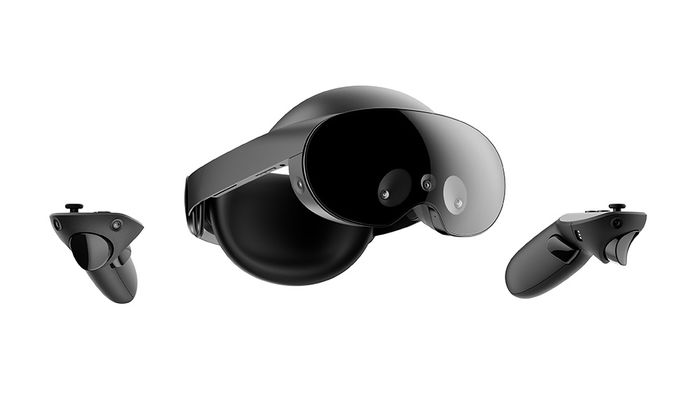
\includegraphics[width=\linewidth, height = 4cm]{img/chapter03/Meta_Quest_Pro.png}
            \caption{Oculus Meta Quest Pro}
            \label{fig:Oculus_Meta_Quest_Pro}
        \end{subfigure}
        \begin{subfigure}[b]{0.45\linewidth}
            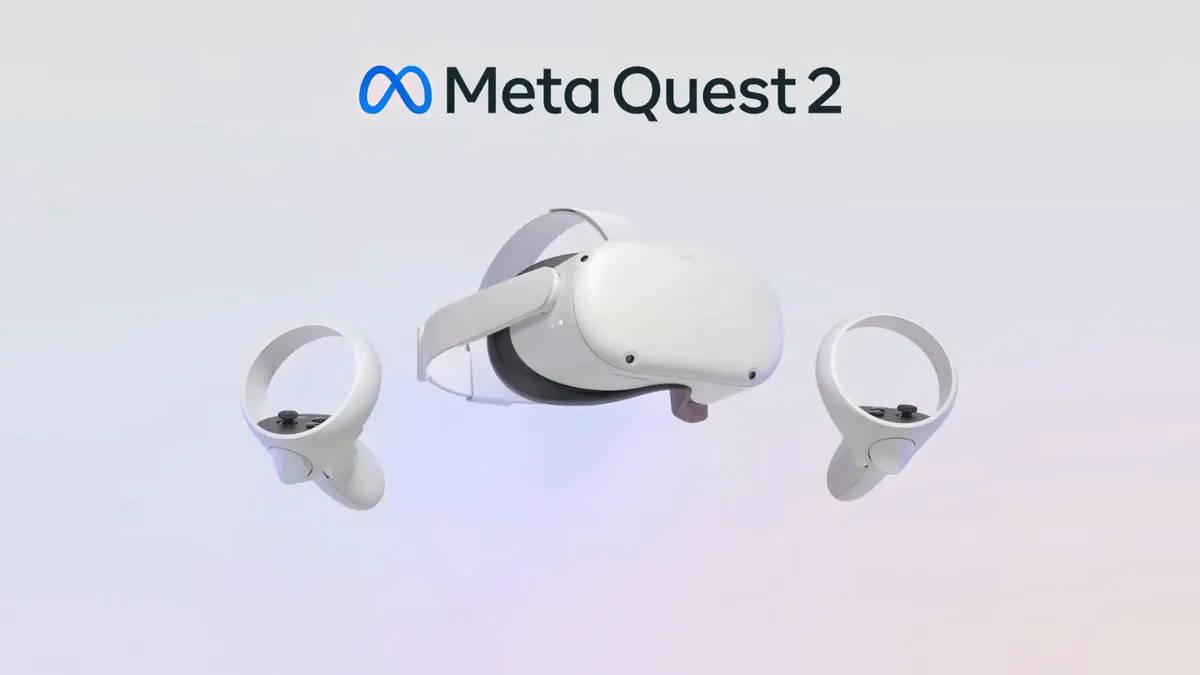
\includegraphics[width=\linewidth, height = 4cm]{img/chapter03/Meta_Quest_2.png}
            \caption{Oculus Meta Quest 2}
            \label{fig:Oculus_Meta_Quest_2}
        \end{subfigure}
        \caption{Sistemas Compatibles}
    \end{figure}
\end{itemize}

\begin{table}[H]
  \centering
  \begin{tabular}{|>{\centering\arraybackslash}m{.5\textwidth}|>{\centering\arraybackslash}m{.3\textwidth}|}
    \hline
    \rowcolor{blue_escom}
     \textbf{Objeto} & \textbf{Costo} \\
     \hline
     Laptop MSI Katana 15 B12V & \$25,440.00\\
     Oculus Meta Quest Pro & \$20,000.00\\
     Oculus Meta Quest 2 & \$10,000.00\\
     \hline
     \rowcolor{column_color}
     \textbf{Total} & \$55,440.00\\
     \hline
  \end{tabular}
  \caption{Costos de Infraestructura}
  \label{tab:Costos}
\end{table}

\textit{\textbf{Licenciamiento}}

Se incluyen las licencias y herramientas externas necesarias para el desarrollo, como se detalla en la \autoref{tab:Licencias}.
\begin{table}[H]
  \centering
  \begin{tabular}{|>{\centering\arraybackslash}m{.5\textwidth}|>{\centering\arraybackslash}m{.3\textwidth}|}
    \hline
    \rowcolor{blue_escom}
     \textbf{Licenciamiento} & \textbf{Costo}\\
     \hline
     Unity Assets & \$5,000.00\\
     SPEECHGEN.IO & \$600.00\\
     3D & \$500.00\\
     \hline
     \rowcolor{column_color}
     \textbf{Total} & \$6,100.00\\
     \hline
  \end{tabular}
  \caption{Costos de Licencias}
  \label{tab:Licencias}
\end{table}

\textit{\textbf{Gastos de Operación}}

Se estimaron gastos operativos aproximados de \$11,000.00 MXN.

El costo total del sistema se calcula sumando todos los conceptos anteriores:

\begin{center}
    \textit{\textbf{Costos del sistema} = Mano de obra + Equipo de Desarrollo + Licenciamiento + Gastos de Operación}
    
    \textit{\textbf{Costo del sistema} = \$46,200.00 + \$55,440.00 + \$6,100.00 + \$11,000.00}
    
    \textit{\textbf{Costo del sistema} = \$118,300.00 MXN}
\end{center}

Este costo incluye la curva de aprendizaje asociada con el desarrollo inicial. Si el proyecto se repitiera desde cero con la necesidad de adquirir nuevamente la infraestructura y las licencias, pero considerando que el tiempo requerido sería la mitad, el costo total estimado se reduciría aproximadamente a \$95,200.00 MXN. En caso de contar ya con toda la infraestructura y las licencias necesarias, el costo total disminuiría aún más, alcanzando aproximadamente \$34,100.00 MXN.

\section{Modelado del Sistema}
\subsection{Casos de Uso}
\begin{figure}[H]
    \centering
    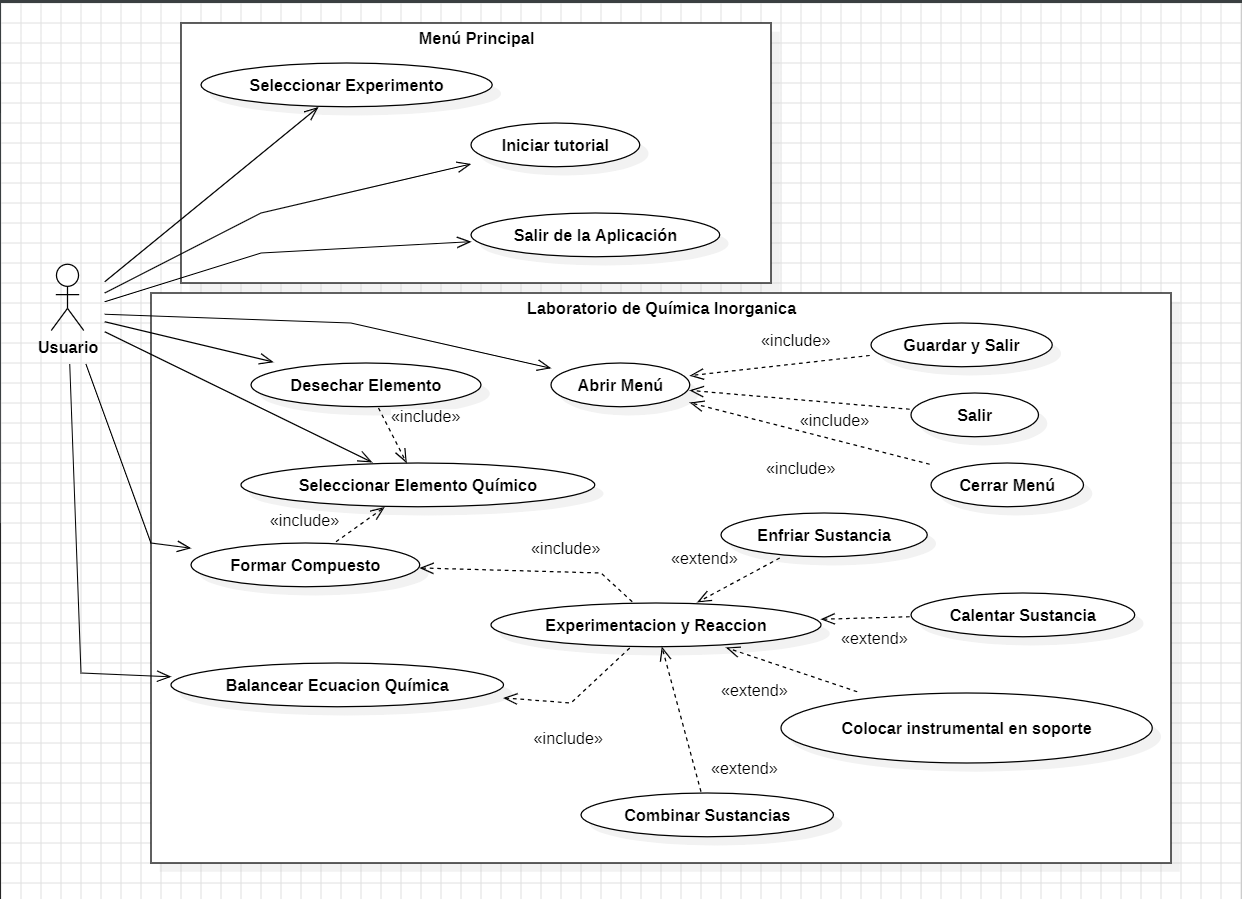
\includegraphics[width=1\textwidth, height=12cm]{img/chapter03/Casos de Uso.png}
    \caption{Diagrama de casos de uso para el sistema}\label{fig:Casos de Uso}
\end{figure}
\newpage
\begin{longtable}{>{\raggedright\arraybackslash}m{.25\textwidth} >{\raggedright\arraybackslash}m{.65\textwidth}}
    \toprule\toprule
    \textbf{Caso de Uso} & Seleccionar Experimento \\
    \midrule\midrule
    \endfirsthead

    \toprule\toprule
    \textbf{Caso de Uso} & Seleccionar Experimento \\
    \midrule\midrule
    \endhead

    \midrule
    \multicolumn{2}{r}{\textit{Continúa en la siguiente página}} \\
    \midrule
    \endfoot

    \endlastfoot

    \textbf{Descripción corta} & El usuario elige un experimento de química para realizar en el simulador. \\
    \midrule
    \textbf{Precondición} & El usuario se encuentra en el menú principal del simulador. \\
    \midrule
    \textbf{Postcondición} & El sistema carga el entorno y los materiales del experimento seleccionado, y presenta al usuario las instrucciones iniciales. \\
    \midrule
    \textbf{Situaciones de error} & \textbf{Selección Inválida:} El usuario intenta seleccionar un experimento que no existe o no está disponible.  \\
    \midrule
    \textbf{Actores} & Usuario \\
    \midrule
    \textbf{Disparadores} & El usuario interactúa con la interfaz del menú principal y selecciona un experimento de la lista. \\
    \midrule
    \textbf{Proceso estándar} &
    \begin{enumerate}
        \item El sistema muestra una lista de experimentos disponibles en el menú principal. 
        \item El usuario utiliza el hand tracking para seleccionar un experimento de la lista. 
        \item El sistema verifica la validez de la selección. 
        \item El sistema carga el entorno virtual del laboratorio, incluyendo los materiales y equipos necesarios para el experimento. 
        \item El sistema presenta al usuario las instrucciones iniciales del experimento. 
    \end{enumerate} \\
    \midrule
    \textbf{Procesos alternativos} & \textbf{3A. Selección Inválida: }
    \begin{enumerate}
        \item El sistema detecta que la selección del usuario no es válida.
        \item El sistema muestra un mensaje de error indicando que el experimento no existe o no está disponible.
        \item El sistema regresa al menú principal.
    \end{enumerate}\\
    \midrule
    \caption{Descripción del caso de uso Seleccionar Experimento}
    \label{tab:Caso_de_uso_Seleccionar_Experimento}
\end{longtable}

\begin{longtable}{>{\raggedright\arraybackslash}m{.25\textwidth} >{\raggedright\arraybackslash}m{.65\textwidth}}
    \toprule\toprule
    \textbf{Caso de Uso} & Iniciar Tutorial \\
    \midrule\midrule
    \endfirsthead

    \toprule\toprule
    \textbf{Caso de Uso} & Iniciar Tutorial \\
    \midrule\midrule
    \endhead

    \midrule
    \multicolumn{2}{r}{\textit{Continúa en la siguiente página}} \\
    \midrule
    \endfoot

    \endlastfoot

    \textbf{Descripción corta} &El usuario accede a un tutorial interactivo para aprender a utilizar las funciones básicas del simulador. \\
    \midrule
    \textbf{Precondición} & El usuario se encuentra en el menú principal del simulador. \\
    \midrule
    \textbf{Postcondición} & El usuario ha completado el tutorial y está familiarizado con las interacciones básicas del simulador. \\
    \midrule
    \textbf{Situaciones de error} & No aplica.  \\
    \midrule
    \textbf{Actores} & Usuario \\
    \midrule
    \textbf{Disparadores} & El usuario selecciona la opción Iniciar Tutorial en el menú principal.\\
    \midrule
    \textbf{Proceso estándar} &
    \begin{enumerate}
        \item El sistema presenta una serie de instrucciones y demostraciones interactivas que guían al usuario a través de las funciones básicas del simulador, como la selección de elementos de la tabla periódica, la manipulación de objetos y la realización de mediciones. 
        \item El usuario sigue las instrucciones y completa las tareas interactivas utilizando el hand tracking. 
        \item El sistema proporciona retroalimentación visual y auditiva al usuario sobre su desempeño en cada tarea. 
        \item Una vez completadas todas las tareas del tutorial, el sistema regresa al menú principal.  
    \end{enumerate} \\
    \midrule
    \textbf{Procesos alternativos} & No aplica.\\
    \midrule
    \caption{Descripción del caso de uso Iniciar Tutorial}
    \label{tab:Caso_de_uso_Iniciar_Tutorial}
\end{longtable}

\begin{longtable}{>{\raggedright\arraybackslash}m{.25\textwidth} >{\raggedright\arraybackslash}m{.65\textwidth}}
    \toprule\toprule
    \textbf{Caso de Uso} &  Balancear Ecuación Química \\
    \midrule\midrule
    \endfirsthead

    \toprule\toprule
    \textbf{Caso de Uso} &  Balancear Ecuación Química \\
    \midrule\midrule
    \endhead

    \midrule
    \multicolumn{2}{r}{\textit{Continúa en la siguiente página}} \\
    \midrule
    \endfoot

    \endlastfoot

    \textbf{Descripción corta} & El usuario balancea una ecuación química proporcionada por el sistema. \\
    \midrule
    \textbf{Precondición} & El sistema ha presentado al usuario una ecuación química desbalanceada como parte de un experimento. \\
    \midrule
    \textbf{Postcondición} & El usuario ha balanceado correctamente la ecuación química, y el sistema lo verifica y permite avanzar al siguiente paso del experimento.  \\
    \midrule
    \textbf{Situaciones de error} & \textbf{Balanceo Incorrecto:} El usuario intenta confirmar un balanceo incorrecto de la ecuación.   \\
    \midrule
    \textbf{Actores} & Usuario \\
    \midrule
    \textbf{Disparadores} & El sistema presenta una ecuación química desbalanceada y solicita al usuario que la balancee.\\
    \midrule
    \textbf{Proceso estándar} &
    \begin{enumerate}
        \item El sistema muestra la ecuación química desbalanceada en la interfaz de usuario. 
        \item El usuario utiliza el hand tracking para interactuar con los coeficientes de la ecuación, incrementándolos o decrementándolos según sea necesario. 
        \item El usuario confirma que ha terminado de balancear la ecuación. 
        \item El sistema verifica si la ecuación está balanceada correctamente. 
        \item Si la ecuación está balanceada, el sistema permite al usuario avanzar al siguiente paso del experimento.  
    \end{enumerate} \\
    \midrule
    \textbf{Procesos alternativos} & 4A. \textbf{Balanceo Incorrecto: }
    \begin{itemize}
        \item El sistema detecta que la ecuación no está balanceada correctamente. 
        \item El sistema muestra un mensaje de error indicando que el balanceo es incorrecto. 
        \item El sistema permite al usuario seguir intentando balancear la ecuación. 
    \end{itemize}\\
    \midrule
    \caption{Descripción del caso de uso  Balancear Ecuación Química}
    \label{tab:Caso_de_uso_ Balancear_Ecuación_Química}
\end{longtable}

\begin{longtable}{>{\raggedright\arraybackslash}m{.25\textwidth} >{\raggedright\arraybackslash}m{.65\textwidth}}
    \toprule\toprule
    \textbf{Caso de Uso} &  Seleccionar Elemento Químico \\
    \midrule\midrule
    \endfirsthead

    \toprule\toprule
    \textbf{Caso de Uso} &  Seleccionar Elemento Químico \\
    \midrule\midrule
    \endhead

    \midrule
    \multicolumn{2}{r}{\textit{Continúa en la siguiente página}} \\
    \midrule
    \endfoot

    \endlastfoot

    \textbf{Descripción corta} &  El usuario selecciona un elemento químico de la tabla periódica interactiva.  \\
    \midrule
    \textbf{Precondición} & La tabla periódica interactiva está visible en la interfaz del usuario.  \\
    \midrule
    \textbf{Postcondición} & 
    \begin{itemize}
        \item El elemento seleccionado se resalta visualmente en la tabla periódica. 
        \item Se muestra información detallada sobre el elemento seleccionado en una interfaz separada. 
        \item Se genera un modelo 3D del elemento seleccionado en el área de trabajo. 
    \end{itemize}\\
    \midrule
    \textbf{Situaciones de error} & No aplica. \\
    \midrule
    \textbf{Actores} & Usuario \\
    \midrule
    \textbf{Disparadores} & El usuario toca un elemento químico en la tabla periódica interactiva utilizando el hand tracking.\\
    \midrule
    \textbf{Proceso estándar} &
    \begin{enumerate}
        \item El usuario toca un elemento químico en la tabla periódica interactiva. 
        \item El sistema detecta la selección y resalta visualmente el elemento. 
        \item El sistema recupera información detallada sobre el elemento seleccionado (nombre, símbolo, número atómico, masa atómica, etc.) y la muestra en una interfaz de usuario separada. 
        \item El sistema genera un modelo 3D del elemento seleccionado y lo coloca en el área de trabajo.  
    \end{enumerate} \\
    \midrule
    \textbf{Procesos alternativos} & No aplica. \\
    \midrule
    \caption{Descripción del caso de uso  Seleccionar Elemento Químico}
    \label{tab:Caso_de_uso_ Balancear_Seleccionar_Elemento_Químico}
\end{longtable}

\begin{longtable}{>{\raggedright\arraybackslash}m{.25\textwidth} >{\raggedright\arraybackslash}m{.65\textwidth}}
    \toprule\toprule
    \textbf{Caso de Uso} &  Crear Compuesto \\
    \midrule\midrule
    \endfirsthead

    \toprule\toprule
    \textbf{Caso de Uso} &  Crear Compuesto \\
    \midrule\midrule
    \endhead

    \midrule
    \multicolumn{2}{r}{\textit{Continúa en la siguiente página}} \\
    \midrule
    \endfoot

    \endlastfoot

    \textbf{Descripción corta} &  El usuario crea un compuesto químico combinando elementos seleccionados de la tabla periódica. \\
    \midrule
    \textbf{Precondición} & 
    \begin{itemize}
        \item El usuario ha seleccionado los elementos químicos necesarios para formar el compuesto. 
        \item Los elementos seleccionados están presentes en el área de trabajo. 
    \end{itemize}\\
    \midrule
    \textbf{Postcondición} & 
    \begin{itemize}
        \item El sistema genera un modelo 3D del compuesto formado. 
        \item El modelo 3D del compuesto se coloca en el área de trabajo. 
        \item Los modelos 3D de los elementos utilizados se eliminan del área de trabajo. 
    \end{itemize}\\
    \midrule
    \textbf{Situaciones de error} & 
    \begin{itemize}
        \item \textbf{Combinación Inválida: }El usuario intenta combinar elementos que no forman un compuesto válido. 
        \item \textbf{Elementos Insuficientes: }El usuario no ha seleccionado todos los elementos necesarios para formar el compuesto. 
    \end{itemize}\\
    \midrule
    \textbf{Actores} & Usuario \\
    \midrule
    \textbf{Disparadores} & El usuario toca un elemento químico en la tabla periódica interactiva utilizando el hand tracking.\\
    \midrule
    \textbf{Proceso estándar} &
    \begin{enumerate}
        \item El usuario indica al sistema que desea crear un compuesto. 
        \item El sistema verifica si la combinación de elementos es válida y si todos los elementos necesarios están presentes. 
        \item Si la combinación es válida, el sistema genera un modelo 3D del compuesto y lo coloca en el área de trabajo. 
        \item El sistema elimina los modelos 3D de los elementos utilizados.  
    \end{enumerate} \\
    \midrule
    \textbf{Procesos alternativos} & 
    \begin{enumerate}[{2}A. ]
        \item \textbf{Combinación Inválida: }
        \begin{itemize}
            \item El sistema detecta que la combinación de elementos no es válida. 
            \item El sistema muestra un mensaje de error indicando que la combinación no es posible. 
            \item El sistema permite al usuario seleccionar otros elementos o cancelar la creación del compuesto.
        \end{itemize}
        \item \textbf{Elementos Insuficientes: }
        \begin{itemize}
            \item El sistema detecta que faltan elementos para formar el compuesto. 
            \item El sistema muestra un mensaje de error indicando los elementos faltantes. 
            \item El sistema permite al usuario seleccionar los elementos faltantes o cancelar la creación del compuesto. 
        \end{itemize}      
    \end{enumerate}\\
    \midrule
    \caption{Descripción del caso de uso Crear Compuesto}
    \label{tab:Caso_de_uso_ Balancear_Crear_Compuesto}
\end{longtable}

\begin{longtable}{>{\raggedright\arraybackslash}m{.25\textwidth} >{\raggedright\arraybackslash}m{.65\textwidth}}
    \toprule\toprule
    \textbf{Caso de Uso} &   Calentar Compuesto \\
    \midrule\midrule
    \endfirsthead

    \toprule\toprule
    \textbf{Caso de Uso} &   Calentar Compuesto \\
    \midrule\midrule
    \endhead

    \midrule
    \multicolumn{2}{r}{\textit{Continúa en la siguiente página}} \\
    \midrule
    \endfoot

    \endlastfoot

    \textbf{Descripción corta} &  El usuario calienta un compuesto utilizando un mechero Bunsen. \\
    \midrule
    \textbf{Precondición} & 
    \begin{itemize}
        \item El mechero Bunsen está disponible y encendido. 
        \item El usuario se encuentra en una etapa del experimento que requiere calentar un compuesto. 
    \end{itemize}\\
    \midrule
    \textbf{Postcondición} &  El compuesto válido se calienta y se muestran los cambios visuales y auditivos correspondientes.\\
    \midrule
    \textbf{Situaciones de error} & El usuario intenta calentar una sustancia o compuesto no válido.\\
    \midrule
    \textbf{Actores} & Usuario \\
    \midrule
    \textbf{Disparadores} & El usuario acerca el compuesto al mechero Bunsen.\\
    \midrule
    \textbf{Proceso estándar} &
    \begin{enumerate}
        \item El usuario selecciona el mechero Bunsen y lo acerca a la sustancia o compuesto (Controlador). 
        \item El sistema verifica si la sustancia o compuesto es válido para calentar (Modelo). 
        \item Si es válido, el sistema detecta la proximidad y activa el calentamiento (Modelo). 
        \item El sistema simula el efecto del calor en el compuesto, mostrando cambios visuales (burbujas, cambio de color) y auditivos (sonido de ebullición) (Vista). 
    \end{enumerate} \\
    \midrule
    \textbf{Procesos alternativos} & 
    \begin{enumerate}[{2}A. ]
        \item \textbf{Sustancia o Compuesto No Válido:} Si la sustancia o compuesto no es válido, el sistema muestra un mensaje de error.     
    \end{enumerate}\\
    \midrule
    \caption{Descripción del caso de uso Calentar Compuesto}
    \label{tab:Caso_de_uso_ Balancear_Calentar_Compuesto}
\end{longtable}

\begin{longtable}{>{\raggedright\arraybackslash}m{.25\textwidth} >{\raggedright\arraybackslash}m{.65\textwidth}}
    \toprule\toprule
    \textbf{Caso de Uso} &   Enfriar Compuesto \\
    \midrule\midrule
    \endfirsthead

    \toprule\toprule
    \textbf{Caso de Uso} &   Enfriar Compuesto \\
    \midrule\midrule
    \endhead


    \endfoot

    \endlastfoot
    \textbf{Descripción corta} &  El usuario sumerge un vaso de precipitados que contiene una solución en un baño de agua para disminuir su temperatura y observar los cambios resultantes. \\
    \midrule
    \textbf{Precondición} & 
    \begin{itemize}
        \item El vaso de precipitados con la solución a enfriar está presente en el área de trabajo. 
        \item El baño de agua está disponible. 
        \item El usuario se encuentra en una etapa del experimento que requiere enfriar la solución 
    \end{itemize}\\
    \midrule
    \textbf{Postcondición} &  El compuesto válido se enfría y se muestran los cambios visuales correspondientes.\\
    \midrule
    \textbf{Situaciones de error} & El usuario intenta enfriar una sustancia o compuesto no válido.\\
    \midrule
    \textbf{Actores} & Usuario \\
    \midrule
    \textbf{Disparadores} & El usuario acerca el recipiente al baño de agua.\\
    \midrule
    \textbf{Proceso estándar} &
    \begin{enumerate}
        \item El usuario selecciona el recipiente que contiene el compuesto y lo sumerge en el baño de hielo (Controlador). 
        \item El sistema verifica si la sustancia o compuesto es válido para enfriar (Modelo). 
        \item Si es válido, el sistema detecta la inmersión y activa el enfriamiento (Modelo). 
        \item El sistema simula el efecto del enfriamiento en el compuesto (Vista).  
    \end{enumerate} \\
    \midrule
    \textbf{Procesos alternativos} & 
    \begin{enumerate}[{2}A. ]
        \item \textbf{Sustancia o Compuesto No Válido:} Si la sustancia o compuesto no es válido, el sistema muestra un mensaje de error. 
    \end{enumerate}\\
    \midrule
    \caption{Descripción del caso de uso Enfriar Compuesto}
    \label{tab:Caso_de_uso_ Balancear_Enfriar_Compuesto}
\end{longtable}

\begin{longtable}{>{\raggedright\arraybackslash}m{.25\textwidth} >{\raggedright\arraybackslash}m{.65\textwidth}}
    \toprule\toprule
    \textbf{Caso de Uso} &   Combinar Sustancias \\
    \midrule\midrule
    \endfirsthead

    \toprule\toprule
    \textbf{Caso de Uso} &   Combinar Sustancias \\
    \midrule\midrule
    \endhead

    \midrule
    \multicolumn{2}{r}{\textit{Continúa en la siguiente página}} \\
    \midrule
    \endfoot

    \endlastfoot

    \textbf{Descripción corta} & El usuario combina dos o más sustancias en un nuevo recipiente para iniciar una reacción química.\\
    \midrule
    \textbf{Precondición} & Las sustancias a combinar están disponibles en el área de trabajo.\\
    \midrule
    \textbf{Postcondición} & Las sustancias válidas se combinan en un nuevo recipiente y se produce la reacción química, mostrando los cambios visuales y auditivos correspondientes.\\
    \midrule
    \textbf{Situaciones de error} & El usuario intenta combinar sustancias no válidas.\\
    \midrule
    \textbf{Actores} & Usuario \\
    \midrule
    \textbf{Disparadores} & El usuario arrastra las sustancias seleccionadas a un nuevo recipiente.\\
    \midrule
    \textbf{Proceso estándar} &
    \begin{enumerate}
        \item El usuario selecciona las sustancias que desea combinar y las arrastra al recipiente (Controlador). 
        \item El sistema verifica la validez de las sustancias para ser combinadas (Modelo). 
        \item Si son compatibles, el sistema simula la combinación y la reacción química, mostrando cambios visuales y auditivos (Vista).  
    \end{enumerate} \\
    \midrule
    \textbf{Procesos alternativos} & 
    \begin{enumerate}[{2}A. ]
        \item \textbf{Combinación Inválida:} Si las sustancias no son compatibles, el sistema muestra un mensaje de error.
    \end{enumerate}\\
    \midrule
    \caption{Descripción del caso de uso Combinar Sustancias}
    \label{tab:Caso_de_uso_ Balancear_Combinar_Sustancias}
\end{longtable}

\begin{longtable}{>{\raggedright\arraybackslash}m{.25\textwidth} >{\raggedright\arraybackslash}m{.65\textwidth}}
    \toprule\toprule
    \textbf{Caso de Uso} & Desechar elemento \\
    \midrule\midrule
    \endfirsthead

    \toprule\toprule
    \textbf{Caso de Uso} & Desechar elemento \\
    \midrule\midrule
    \endhead

    \midrule
    \multicolumn{2}{r}{\textit{Continúa en la siguiente página}} \\
    \midrule
    \endfoot

    \endlastfoot

    \textbf{Descripción corta} & El usuario elimina un elemento del área de trabajo.\\
    \midrule
    \textbf{Precondición} & 
    \begin{itemize}
        \item \textbf{Existencia del Elemento:} El elemento a desechar debe estar presente y visible en el área de trabajo.
        \item \textbf{Área de Desecho Habilitada:} El área de desecho debe estar habilitada y accesible para el usuario.
    \end{itemize}\\
    \midrule
    \textbf{Postcondición} & El elemento o compuesto se elimina del área de trabajo.\\
    \midrule
    \textbf{Situaciones de error} & El usuario intenta desechar un elemento que el sistema no permite eliminar en ese momento del experimento.\\
    \midrule
    \textbf{Actores} & Usuario \\
    \midrule
    \textbf{Disparadores} &  El usuario deposita el elemento en el área de desecho.\\
    \midrule
    \textbf{Proceso estándar} &
    \begin{enumerate}
        \item \textbf{Inicio:} El usuario toma el elemento o compuesto a desechar.
        \item \textbf{Movimiento}: El usuario mueve el elemento o compuesto hacia el área de desecho.
        \item \textbf{Soltar:} El usuario suelta el elemento o compuesto dentro de los límites del área de desecho.
        \item \textbf{Validación:} El sistema valida que el elemento o compuesto puede ser desechado en ese momento del experimento.
        \item \textbf{Eliminación:} El sistema elimina el elemento o compuesto del área de trabajo y de cualquier estructura de datos asociada.
    \end{enumerate} \\
    \midrule
    \textbf{Procesos alternativos} & 
    \begin{enumerate}[{4}A. ]
        \item Validación: El sistema detecta que el elemento o compuesto no puede ser desechado en ese momento.
        \item Notificación: El sistema muestra un mensaje de error claro indicando que el elemento o compuesto no puede ser desechado en ese momento.
        \item Cancelación: El elemento o compuesto regresa a su posición original en el área de trabajo.
    \end{enumerate}\\
    \midrule
    \caption{Descripción del caso de uso Desechar elemento}
    \label{tab:Caso_de_uso_ Balancear_Desechar_elemento}
\end{longtable}

\begin{longtable}{>{\raggedright\arraybackslash}m{.25\textwidth} >{\raggedright\arraybackslash}m{.65\textwidth}}
    \toprule\toprule
    \textbf{Caso de Uso} & Experimentación y Reacción \\
    \midrule\midrule
    \endfirsthead

    \toprule\toprule
    \textbf{Caso de Uso} & Experimentación y Reacción \\
    \midrule\midrule
    \endhead

    \midrule
    \multicolumn{2}{r}{\textit{Continúa en la siguiente página}} \\
    \midrule
    \endfoot

    \endlastfoot

    \textbf{Descripción corta} & El usuario interactúa con los compuestos y el instrumental para realizar la experimentación y reacción química, mientras el sistema simula los efectos.\\
    \midrule
    \textbf{Precondición} & 
    \begin{itemize}
        \item \textbf{Compuestos disponibles:} Los compuestos químicos necesarios para el experimento se seleccionaron y están en el área de trabajo virtual.
        \item \textbf{Instrumental disponible: }El instrumental virtual requerido (matraces, pipetas, mecheros, etc.) está presente y accesible en el área de trabajo.
    \end{itemize}\\
    \midrule
    \textbf{Postcondición} & 
    \begin{itemize}
        \item \textbf{Resultados simulados:} El sistema ha simulado los resultados de la reacción o experimento químico realizado por el usuario.
        \item \textbf{Visualización de resultados:} El usuario puede observar los cambios en los compuestos, la formación de nuevos productos, cambios de temperatura, etc., en la interfaz del sistema.
    \end{itemize}\\
    \midrule
    \textbf{Situaciones de error} & 
    \begin{itemize}
        \item \textbf{Compuestos Insuficientes:} El usuario intenta realizar un experimento sin todos los compuestos necesarios.
        \item \textbf{Acciones Inválidas:} Si el usuario intenta realizar una acción no permitida por el diseño del experimento, el sistema lo notificará y detendrá la simulación.
    \end{itemize}\\
    \midrule
    \textbf{Actores} & Usuario \\
    \midrule
    \textbf{Disparadores} &  El usuario comienza a interactuar con los compuestos o el instrumental virtual.\\
    \midrule
    \textbf{Proceso estándar} &
    \begin{enumerate}
        \item \textbf{Inicio:} El usuario toma el elemento o compuesto a desechar.
        \item \textbf{Movimiento}: El usuario mueve el elemento o compuesto hacia el área de desecho.
        \item \textbf{Soltar:} El usuario suelta el elemento o compuesto dentro de los límites del área de desecho.
        \item \textbf{Validación:} El sistema valida que el elemento o compuesto puede ser desechado en ese momento del experimento.
        \item \textbf{Eliminación:} El sistema elimina el elemento o compuesto del área de trabajo y de cualquier estructura de datos asociada.
    \end{enumerate} \\
    \midrule
    \textbf{Procesos alternativos} & 
    \begin{enumerate}[{4}A. ]
        \item Validación: El sistema detecta que el elemento o compuesto no puede ser desechado en ese momento.
        \item Notificación: El sistema muestra un mensaje de error claro indicando que el elemento o compuesto no puede ser desechado en ese momento.
        \item Cancelación: El elemento o compuesto regresa a su posición original en el área de trabajo.
    \end{enumerate}\\
    \midrule
    \caption{Descripción del caso de uso Experimentación y Reacción}
    \label{tab:Caso_de_uso_ Balancear_Experimentación_y_Reacción}
\end{longtable}

\begin{longtable}{>{\raggedright\arraybackslash}m{.25\textwidth} >{\raggedright\arraybackslash}m{.65\textwidth}}
    \toprule\toprule
    \textbf{Caso de Uso} & Main Menu \\
    \midrule\midrule
    \endfirsthead

    \toprule\toprule
    \textbf{Caso de Uso} & Main Menu \\
    \midrule\midrule
    \endhead

    \midrule
    \multicolumn{2}{r}{\textit{Continúa en la siguiente página}} \\
    \midrule
    \endfoot

    \endlastfoot

    \textbf{Descripción corta} &El usuario sale del experimento actual y regresa al menú de bienvenida. \\
    \midrule
    \textbf{Precondición} & El usuario se encuentra en el Menú del escenario de un experimento.\\
    \midrule
    \textbf{Postcondición} &  El experimento actual se cierra y el usuario regresa al menú de bienvenida. \\
    \midrule
    \textbf{Situaciones de error} & Ninguna\\
    \midrule
    \textbf{Actores} & Usuario \\
    \midrule
    \textbf{Disparadores} & El usuario selecciona la opción "Main Menu" en el menú.\\
    \midrule
    \textbf{Proceso estándar} &
    \begin{enumerate}
        \item El sistema detecta la selección de la opción "Main Menu".
        \item El sistema detiene la simulación del experimento actual.
        \item El sistema regresa al menú de bienvenida.
    \end{enumerate} \\
    \midrule
    \textbf{Procesos alternativos} & Ninguno.\\
    \midrule
    \caption{Descripción del caso de uso Main Menu}
    \label{tab:Caso_de_uso_Main_Menu}
\end{longtable}

\begin{longtable}{>{\raggedright\arraybackslash}m{.25\textwidth} >{\raggedright\arraybackslash}m{.65\textwidth}}
    \toprule\toprule
    \textbf{Caso de Uso} & Colocar instrumental en soporte \\
    \midrule\midrule
    \endfirsthead

    \toprule\toprule
    \textbf{Caso de Uso} & Colocar instrumental en soporte\\
    \midrule\midrule
    \endhead

    \midrule
    \multicolumn{2}{r}{\textit{Continúa en la siguiente página}} \\
    \midrule
    \endfoot

    \endlastfoot

    \textbf{Descripción corta} &El usuario coloca un instrumento de laboratorio en un soporte designado. \\
    \midrule
    \textbf{Precondición} & El usuario está sosteniendo un instrumento de laboratorio con la mano y hay un soporte disponible.\\
    \midrule
    \textbf{Postcondición} & El instrumento de laboratorio se coloca en el soporte y se libera de la mano del usuario. \\
    \midrule
    \textbf{Situaciones de error} & No hay un soporte disponible o el usuario no está sosteniendo un instrumento compatible con el soporte. \\
    \midrule
    \textbf{Actores} & Usuario \\
    \midrule
    \textbf{Disparadores} & El usuario acerca el instrumento al soporte y realiza el gesto de "soltar". \\
    \midrule
    \textbf{Proceso estándar} &
    \begin{enumerate}
        \item El sistema detecta que el usuario está acercando un instrumento a un soporte.
        \item El sistema verifica si el soporte está disponible y si el instrumento es compatible.
        \item Si el soporte está disponible y el instrumento es compatible, el sistema coloca el instrumento en el soporte y lo libera de la mano del usuario.
    \end{enumerate} \\
    \midrule
    \textbf{Procesos alternativos} & 3A. Si el soporte no está disponible o el instrumento no es compatible, el sistema muestra un mensaje de error al usuario..\\
    \midrule
    \caption{Descripción del caso de uso Colocar instrumental en soporte}
    \label{tab:Caso_de_uso_Colocar_instrumental_en_soporte}
\end{longtable}
\newpage
\subsection{Diagrama de Clases}
\begin{figure}[thbp]
    \centering
    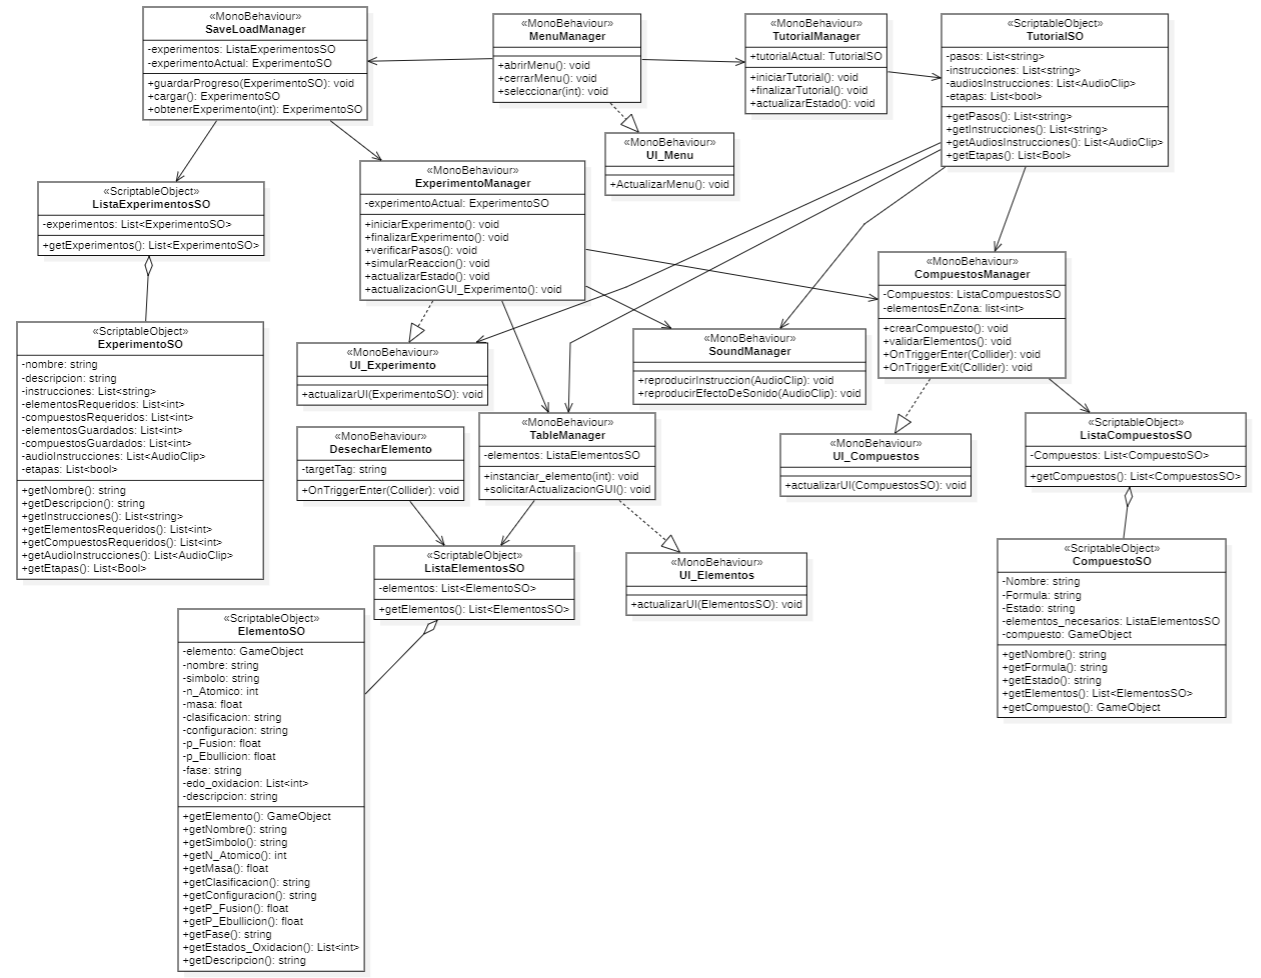
\includegraphics[width=0.9\textwidth, height = 15cm]{img/chapter03/Diagrama de Clases.png}
    \caption{Diagrama de Clases}
    \label{fig:Diagrama_de_Clases}
\end{figure}